\chapter{Senzory}

Senzory k projektu Pletačka IoT jsou postavené na mikročipu ESP32 a moduly TTGO~T-Display.
Celý tento systém je navržen tak, že na každém pletacím stroji je jedna moje elektronika.
Každý z těchto senzorů má svoje jedinečné číslo, pod kterým posílá naměřená data na server.
Senzor je na pájen z 5 nebo 24 voltů a má spotřebu 120 mA.
Návrh senzorů i jejich software mám verzovaný nástrojem Git ve veřejném repozitáři na GitHubu.\newline
GitHub: \href{https://github.com/Pletacka-IoT/Pletacka-board}{Pletacka-board}\cite{PL_BOARD}

\section{1. verze - univerzální sensorika}

První verzi jsem pojal jako testovací. Bylo tedy potřeba navrhnout univerzální desku a otestovat celý systém.\newline

Při navrhování první verze senzoru jsem se držel těmito body:
\begin{itemize}
    \item ESP32 s barevným displejem
    \item vstup ze 4 periferií
    \item vstupní napětí od 10 do 25V
    \item teplotní čidlo
    \item tři barevné diody
    \item čtyři uživatelská tlačítka
\end{itemize}


\subsection{Řídící deska}
Návrh desky jsem tvořil v aplikaci EAGLE od společnosti Autodesk. 
Deska má rozměry 75 na 60 mm a v každém rohu má upevňovací díry. 
Kabely se do desky připojují pomocí 5mm svorkovnice.
Na vstupu napájení je měnič napětí který pracuje v rozsahu od 10 do 25 voltů a na výstupu dává 5V. 

Řídící procesor celé desky je modul ESP32 TTGO T-Display.
Tento čip také zajišťuje WiFi konektivitu s okolím a odesílá naměřená data na server.
Pro univerzální detekování vstupů z periferií se využívají optočleny, které předávají signál do mikroprocesoru.
K uživatelskému ovládání senzoru jsou zde čtyři programovatelná tlačítka a tři indikační diody.
Aktuální naměřená data se zobrazují na displeji a informují obsluhu o zastavení stroje a počtu upletených párů.
Senzor je také schopen zaznamenávat data ze čtyř vstupů a teplotu z teplotního senzoru. Viz obrázek \ref{fig:SenzorV1.0NaStroji}.

\section{Uchycení}
Obal řídící desky je vytisknutý na 3D tiskárně z materiálu PETG.
Na přední straně je průhled z plexi skla na barevný displej a okolo něj jsou rozmístěná uživatelská tlačítka.
Na boční straně krabičky jsou připravené dvě drážky na protažení stahovacích zip pásků pro uchycení na sloupek stroje.
Kabely jsou poté svedeny po konstrukci stroje až k periferiím.


\section{Program}
K programování využívám aplikaci Visual Studio Code s rozšířením PlatformIO, které je navržena k programování mikrokontrolérů. 
Zdrojový kód mám napsaný v jazyce C++.
Program se skládá z několika vláken, které se pravidelně spouštějí a vykonávají.
První a zároveň nejdůležitější vlákno je senzorové, zde se periodicky kontroluje stav periferií a při změně se odešle událost na server.
Další vlákno zajišťuje pravidelné vykreslování dat na displej a zbylá vlákna se starají o správný chod senzoru.
Software také obsahuje ladící mód ve kterém si administrátor může zobrazit stav senzoru v mobilní aplikaci a jednodušeji tak hledat potenciální chybu. 


\fxnote[author=JA]{\textcolor{mygreen}{Obrázek deksa => krabička}}

\begin{figure}[htbp]
    \centering
    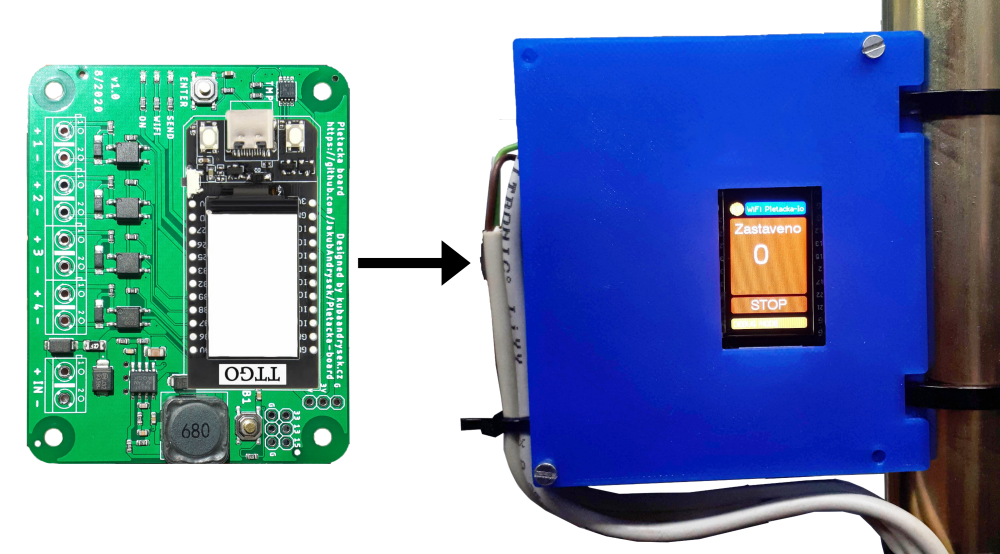
\includegraphics[width=\textwidth]{img/SenzorV1.png}
    \caption{Senzor - 1. verze}
    \label{fig:SenzorV1.0NaStroji}
\end{figure}

\fxnote[author=JPA]{\textcolor{mygreen}{Nevím jestli bych zde nepreferoval pouze obrázek desky bez krabičky + do bílé plochy displeje vložit obraz z fotky s krabičkou => Zastaveno 0...}}
\newpage





% 2. verze - speciální senzorika
\section{2. verze - speciální senzorika}

Po měsíci testování jsem zhodnotil využití jednotlivých součástek a následně jsem vytvořil nový seznam požadavků, přizpůsobený pro lepší chod senzoru.
Zařízení je díky tomu mnohem menší, levnější a softwarově rychlejší.

\begin{itemize}
    \item vstup pouze ze 2 periferií
    \item vstupní napětí již od 5V
    \item zredukování rozměrů
    \item moderní USB-C konektor
    \item zredukování na dvě tlačítka a dvě indikační diody
    \item možnost přímého napájení senzoru bez měniče
\end{itemize}

\subsection{Řídící deska}
Návrh druhé desky jsem se rozhodl udělat v open source aplikaci KiCad.
Tato aplikace podporuje mnoho rozšíření, která velmi zpříjemní návrh a zjednoduší přípravu podkladů.

V novém návrhu jsem se~především zaměřoval na~rozměr desky, ten aktuálně činí 32$\times$76mm, což je o 46 procent menší plocha než u první verze.

Deska si~zachovala stejný procesor ESP32 s~displejem, ale přišla~o dvě~tlačítka a~jednu indikační diodu.
V~senzoru~se také změnilo zapojení měniče napětí, ten nově dokáže pracovat již od~5V, které následně mění na~3,3V.
Na~bočních stranách desky vznikla také nová "křidélka" pro zasunutí~do vylepšeného krytu.


\fxnote[author=JA]{\textcolor{mygreen}{Obrázek deksa => krabička}}

\section{Uchycení}
Druhá verze využívá stejného principu uchycení, jako ta~předchozí. 
Mění se~zde však spojení krabičky se~senzorovou deskou. 
V nové verzi jsem desku navrhl tak, aby se~dala jednoduše zasunout~do kolejnic které jsou předtištěné v~krabičce a~následně zafixovat šroubkem ze~zadní strany.
To~umožňuje jednoduchou montáž~a rychlé připojení.
Tento návrh už~má~také vyřešené zafixování kabelů ke~konstrukci krabičky pomocí 3D tištěných svěrek.


\section{Program}
Program druhé verze vychází z minulé, ale přináší s sebou nové funkce a vylepšuje stávající.
Novou funkcionalitou je například automatická aktualizace programu přes WiFi, kterou nadále zdokonaluji.
Další vylepšení jsem přidal k displeji, který dokáže zobrazit více údajů a automaticky mezi nimi přepínat.

\begin{figure}[htbp]
    \centering
    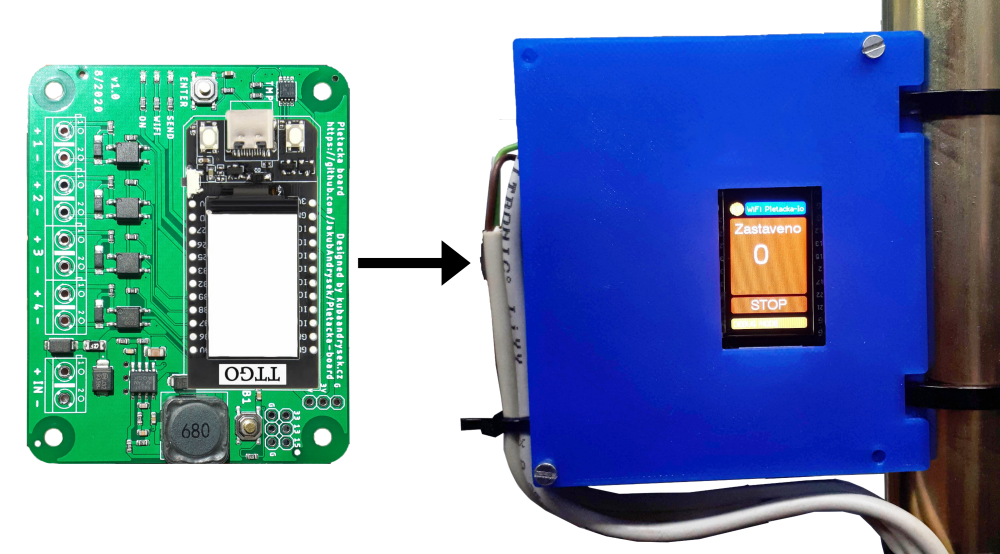
\includegraphics[width=\textwidth]{img/SenzorV1.png}
    \caption{ZDE BUDE 2. verze senzoru}
    \label{fig:SenzorNaStroji}
\end{figure}


\newpage